\documentclass{scrartcl}

\usepackage{amssymb}
\usepackage{amsmath}
\usepackage{tikz}
\usetikzlibrary{calc,intersections,through,backgrounds,patterns}
\usetikzlibrary{decorations.text, decorations.markings, fit, arrows, arrows.meta}

%from Jung - Aion: Researches into the Phenomenology of the Self (1959), pp. 257-60

\begin{document}
	
	%\begin{figure}
	%	\centering
	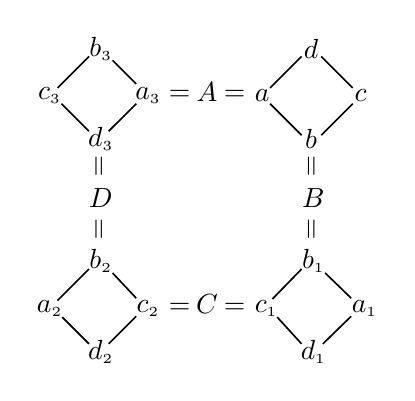
\begin{tikzpicture}
	\node at  (0,1.35) {$A$};
	\node at  (1.35,0) {$B$};
	\node at (0,-1.35) {$C$};
	\node at (-1.35,0) {$D$};
	
	%A equals signs
	\node at (-0.35,1.3) {=};
	\node at  (0.35,1.3) {=};
	
	%B equals signs
	\node at (1.3, 0.4) {\rotatebox{270}{=}};
	\node at (1.3,-0.4) {\rotatebox{270}{=}};
	
	%C equals signs
	\node at (-0.35,-1.4) {=};
	\node at  (0.35,-1.4) {=};
	
	%D equals signs
	\node at (-1.4, 0.4) {\rotatebox{270}{=}};
	\node at (-1.4,-0.4) {\rotatebox{270}{=}};
	
	%top-left - nodes
	\node at (-1.35,1.9)  {$b_\text{{\tiny 3}}$};
	\node at (-0.75,1.3)  {$a_\text{{\tiny 3}}$};
	\node at (-1.35,0.75) {$d_\text{{\tiny 3}}$};
	\node at (-2,1.3) 	  {$c_\text{{\tiny 3}}$};
	
		%top-left - lines
		\draw[semithick] (-0.9,1.45)--(-1.2,1.75);		%a--b
		\draw[semithick] (-0.9,1.2)--(-1.25,0.85);		%a--d
		\draw[semithick] (-1.9,1.4)--(-1.5,1.8);		%c--b
		\draw[semithick] (-1.85,1.2)--(-1.5,0.85);		%c--d
		
	%top-right - nodes
	\node at (1.32,1.9)  {$d$};
	\node at (1.95,1.3)  {$c$};
	\node at (1.32,0.75) {$b$};
	\node at (0.7,1.3)   {$a$};
	
		%top-right - lines
		\draw[semithick] (0.8,1.4)--(1.2,1.8);		%a--d
		\draw[semithick] (0.8,1.2)--(1.2,0.8);		%a--b
		\draw[semithick] (1.85,1.4)--(1.45,1.8);	%c--d
		\draw[semithick] (1.85,1.2)--(1.45,0.8);	%c--b
	
	%bottom-left - nodes
	\node at (-1.35,-1.95) {$d_\text{{\tiny 2}}$};
	\node at (-0.75,-1.4)  {$c_\text{{\tiny 2}}$};
	\node at (-1.35,-0.8)  {$b_\text{{\tiny 2}}$};
	\node at (-2,-1.4)     {$a_\text{{\tiny 2}}$};
	
		%bottom-left - lines
		\draw[semithick] (-0.9,-1.27)--(-1.2,-0.95);	%c--b
		\draw[semithick] (-0.9,-1.5)--(-1.25,-1.85);	%c--d
		\draw[semithick] (-1.9,-1.3)--(-1.5,-0.9);		%a--b
		\draw[semithick] (-1.84,-1.51)--(-1.5,-1.85);	%a--d
	
	%bottom-right - nodes
	\node at (1.35,-0.8)  {$b_\text{{\tiny 1}}$};
	\node at (2,-1.4) 	  {$a_\text{{\tiny 1}}$};
	\node at (1.35,-1.95) {$d_\text{{\tiny 1}}$};
	\node at (0.75,-1.4)  {$c_\text{{\tiny 1}}$};
	
		%bottom-right - lines
		\draw[semithick] (0.89,-1.51)--(1.2,-1.85);		%c--d
		\draw[semithick] (0.83,-1.28)--(1.2,-0.9);		%c--b
		\draw[semithick] (1.83,-1.5)--(1.47,-1.85);		%a--d
		\draw[semithick] (1.83,-1.27)--(1.5,-0.95);		%a--b
	\end{tikzpicture}
	%	\caption{...}
	%\end{figure}
	
	\vspace{1cm}
	
	%\begin{figure}
	%	\centering
	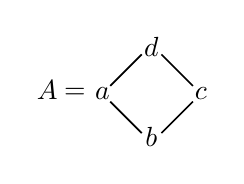
\begin{tikzpicture}
	\node at  (0,0.05) {$A$};
	\node at  (0.35,0) {=};
	
	%nodes
	\node at (1.32,0.6)   {$d$};
	\node at (1.95,0)  	  {$c$};
	\node at (1.32,-0.55) {$b$};
	\node at (0.7,0)	  {$a$};
	
	%lines
	\draw[semithick] (0.8,0.1)--(1.2,0.5);		%a--d
	\draw[semithick] (0.8,-0.1)--(1.2,-0.5);	%a--b
	\draw[semithick] (1.85,0.1)--(1.45,0.5);	%c--d
	\draw[semithick] (1.85,-0.1)--(1.45,-0.5);	%c--b
	
	\end{tikzpicture}
	%	\caption{...}
	%\end{figure}
	
	
\end{document}